\chapter{6. ChainAPI for Air Quality}

ChainAPI \cite{chainGit, chainPaper} is a hypermedia framework for the 'Web of Things'.  It provides a minimal layer of design principles on top of the HAL/JSON specification, to make data sharing and resource addressing simple.  It is extensible-- allowing anyone to define their own ontologies and connect their own data storage solutions in a distributed fashion-- and attempts to only rigorously define a thin, hyperlink layer that allows information to be easily discoverable and easily digestible by any user or service.

\begin{marginfigure}
 	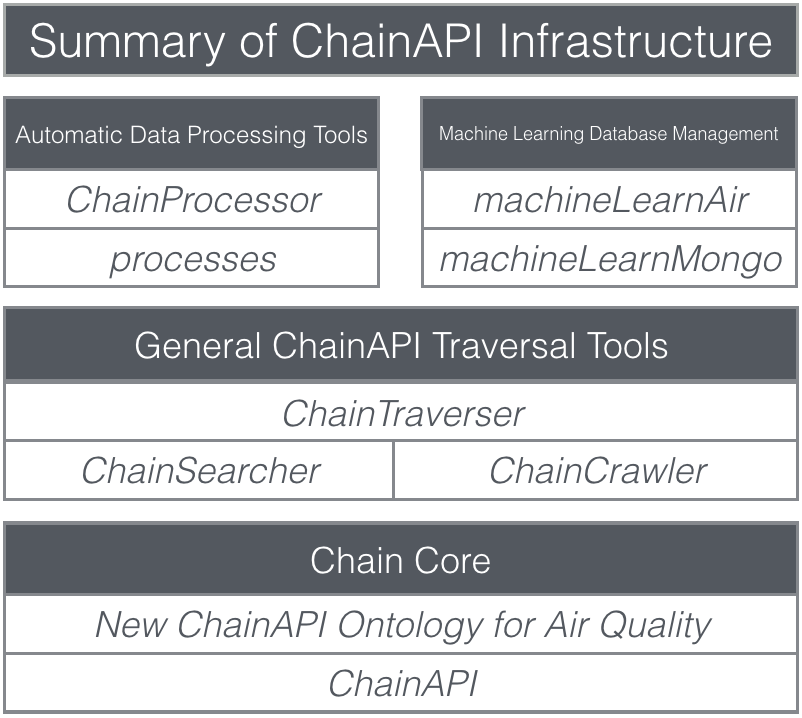
\includegraphics[width=\textwidth]{visuals/chainSummary}               
 	 \caption{Summary of New ChainAPI Infrastructure}
  	\label{fig:chain}
\end{marginfigure}

ChainAPI lends itself to the kinds of problems facing the air quality community.  It allows anyone, with any type of device, to store their data however they see fit, and still easily connect to a broader ecosystem.  It allows researchers to browse through the entire ecosystem like they would the internet.  It incentivizes contribution with a broader data ecosystem and interesting tools, while simultaneously lowering the barrier to entry as much as possible.

In the Responsive Environments group at the MIT Media Lab, ChainAPI already forms the backbone of a large ecological sensor network installation called TidMarsh. \cite{tidmarsh}  It connects hundreds of sensors to a browsable, easy to use backend.  It provides a simple real-time data stream that developers have connected to for building virtual environments, data visualizations, audio compositions, and other novel tools for data interaction.  Besides addressing the core concerns of distributed, scalable, simple data-sharing, ChainAPI also stands as the backbone of several future-looking human interactions and interventions to help individuals live with, understand, internalize, and mediate large datasets.

The TidMarsh ChainAPI environment forms the basis of the ChainAPI Air Quality protocol.  To make it useful for air quality, the first step is to define an ontology that addresses the needs and concerns of the air quality community.  This ontology is significantly larger and more complex than the current ChainAPI ontology, catering specifically to concerns of stationary and mobile air quality sensing.  This includes shared resources that define sensor types and device types and relevant metadata, as well as Organizational and Fixed Site information so that larger groups like the EPA have an example resource that maps well to their current ontology.

While several interesting tools have been created on top of the core ChainAPI for interacting with live streams of known resources, there are no tools to automatically explore and interact with a data ecosystem that is dynamic and growing, or an ecosystem that has reached critical mass (i.e. one update stream becomes infeasible as a way of monitoring all resources).  These are features we would expect from a true, distributed 'Web of Things' solution, and are of particular concern for an air quality installation designed to support deployments ranging from the EPA to small citizen groups.  These features also lay the groundwork for scalable learning algorithms, that can search the network for nearby higher quality sensors and utilize their data.

In this thesis, we define a new ontology for ChainAPI to adapt it to the air quality space.  After creating a development environment that takes advantage of this ontology, we created several tools to enable scalable interaction and advanced learning on this dataset.  These tools-- chainCrawler, chainSearcher, chainTraverser, and chainProcessor-- form a backbone of extensible, powerful options for resource discovery, automatic and transparent cross-organization dataset creation and processing, as well as scalable, advanced machine learning techniques.  It encourages programmatic data processing that can scale and is easily trackable.  It also encourages a separation of concerns-- so the best-in-class raw data collection and the best-in-class pre-processing algorithms can both exist transparently and be applied broadly, instead of siloed researchers batch processing and scrubbing data with opaque techniques before any data is shared.

At it's most advanced, these tools provide a simple way to find and compare co-located sensors of similar type but disparate quality, easily access the conditions under which those measurements occurred, and apply any user-defined algorithm.  This is all scaffolded in such a way that the underlying algorithm or model can simply and automatically update as more data is added to the network.    


\section{A New Ontology for Air Quality}

The first major step in adapting ChainAPI for air quality networks is to define a new ontology.  The basic outline is as follows:

\begin{quote}
\textit{Organizations have Deployments.  Deployments have Fixed Sites and Mobile Devices.  Both Fixed Sites and Mobile Devices have an extensible API datastore for weather conditions, etc. (corresponding to their location) associated with them.  Fixed Sites have (non-Mobile) Devices.  Devices each are associated with a particular Device Type (make and model), and each Device has a collection of Sensors (individual data streams).  Sensors are associated with a particular Sensor Type, and have a collection of SensorData.}
\end{quote}

There are other resources and details, which are outlined in the full documentation below.  Some data (like SensorData, CalibrationData, and APIData) have an associated storage resource that contains general, important information about the collection of data (like what it's measuring, which API it is calling, etc).  LocationData, on the other hand, requires no metadata, and thus does not require a storage resource.  'Type' resources are useful for quickly identifying resources of the same type, and centralizing information about how to handle that type.  

One interesting example of the utility of centralized resource types is that manufacturers could potentially oversee their device and sensor types-- updating metadata and associated calibration algorithms.  A new user to the ChainAPI system could then simply link their sensor resource to the correct type, and an automated crawler could pull the most recent, manufacturer-specified calibrations and apply them automatically to the new user's data.  It could check the conditions under which a measurement was made automatically, and warn the user if the sensor is out of normal operating ranges.  Additionally, the manufacturer could store sensor service information in their sensor type, and have an automated crawler that looks for sensors of that type, checks their serial numbers, and notifies the contact person associated with a resource if their sensor is in need of recalibration.  
   
In general, the principle behind data storage in ChainAPI is to create many 'virtual sensors' to represent one real one.  We encourage users to store raw data in Chain, and after processing it, post the processed data to a parallel 'virtual sensor' that has a name that indicates it comes from the same physical sensor, but has new units or is a new metric. 

A few minutiae are important for interoperability.  Timestamps are stored using ISO8601 standards (timezone aware UTC)-- all python code and scripts will accept (and only accept) one of the major timezone-specified string formats.  Timed/averaged measurements are stored with a 'start time' and a 'duration'.

\begin{lstlisting}[style=codedef]
@@Organization@@
	
	%\textit{An installation of ChainAPI maintained and curated by an Organization.}%

	@@name@@(string) - the name of the organization.
	@@url@@(string) - the website URL associated with the organization.
	@@ch:deployments@@ (related resource) - a collection of deployments associated with the organization.
	@@ch:contacts@@ (related resource) - a collection of contacts associated with the organization.

\end{lstlisting}

\begin{lstlisting}[style=codedef]
@@Deployment@@
	
	%\textit{A particular project owned by an organization, usually with several to hundreds of mobile sensors and/or fixed sites.}%

	@@name@@(string) - the name of the deployment.
	@@geoLocation@@(elevation, latitude, longitude)  - a location to associate with the deployment; usually, the city where the deployment is based.
	@@ch:organization@@ (related resource) - the parent organization.
	@@ch:sites@@ (related resource) - a collection of fixed sites associated with the deployment.
	@@ch:devices@@ (related resource) - a collection of mobile devices associated with the deployment.
	@@ch:contacts@@ (related resource) - a collection of contacts in charge of the deployment.

\end{lstlisting}

\begin{lstlisting}[style=codedef]
@@Fixed Site@@
	
	%\textit{An immovable location where several devices are co-located.}%

	@@name@@(string) - the name/identifier of the site.
	@@url@@(string) - a website URL reference with extra documentation about the site.
	@@geoLocation@@(elevation, latitude, longitude)  - the fixed coordinates/elevation of the site.
	@@ch:deployment@@ (related resource) - the parent deployment.
	@@ch:devices@@ (related resource) - a collection of devices located at the fixed site.
	@@ch:calibration_datastores@@ (related resource) - a collection of calibration datastores associated with the site.
	@@ch:api_datastores@@ (related resource) - a collection of API datastores associated with the site location.	
	@@ch:contacts@@ (related resource) - a collection of contacts in charge of site maintenance.

\end{lstlisting}

\begin{lstlisting}[style=codedef]
@@Device@@
	
	%\textit{A manufactured object that houses a collection of sensors.  If it is mobile, its proper parent is a deployment.  If it is}%
	%\textit{stationary, its proper parent is a fixed site.}%

	@@unique_name@@(string) - a unique identifier for the device.
	@@serial_no@@(string) - the manufacturer's unique identifier for the device.
	@@deploy_date@@(ISO8601 timestamp) - the date the device was put in the field.	
	@@manufacture_date@@(ISO8601 timestamp) - the date the device was manufactured.
	@@description@@(string) - extra, descriptive data pertaining to this device.
	@@ch:device_type@@ (related resource) - general device information for this make/model device.
	@@ch:site@@ (related resource) - the parent site, if a fixed device.
	@@ch:deployment@@ (related resource) - the parent deployment, if a mobile device.
	@@ch:locationDataHistory@@ (related resource) - a collection of timestamped location data, if a mobile device.
	@@ch:api_datastores@@ (related resource) - a collection of API datastores associated with the device's timestamped locationData.
	@@ch:contacts@@ (related resource) - a collection of contacts in charge of the device.
	
\end{lstlisting}

\begin{lstlisting}[style=codedef]
@@Device Type@@
	
	%\textit{A collection of useful data pertaining to several devices of the same make and model.}%

	@@manufacturer@@(string) - the name of the device manufacturer.
	@@model@@(string) - the name/number of the device model.
	@@revision@@(string) - the hardware revision of the device.
	@@datasheet_url@@(string) - the website URL associated with the most current datasheet.
	@@description@@(string) - extra, descriptive data pertaining to this device type.
	@@ch:devices@@ (related resource) - a collection of all devices of this type.

\end{lstlisting}

\begin{lstlisting}[style=codedef]
@@Sensor@@
	
	%\textit{An object that captures a single channel of timestamped data.  There maybe multiple sensors in a device. }%

	@@metric@@(string) - a label for the measured quantity (i.e. 'O3', 'CO', 'NO2').
	@@unit@@(string) - the units of the measurement (i.e. 'ppb', 'ug/m3')
	@@ch:sensor_type@@ (related resource) - general sensor information for this make/model sensor.
	@@dataType@@(string) - the datatype stored by the sensor (float).
	@@value@@(float) - the most recent reading from the sensor.	
	@@updated@@(ISO8601 timestamp) - the timestamp of the most recent reading from the sensor.
	@@ch:dataHistory@@ (related resource) - the collection of timestamped data from this sensor.
	@@ch:device@@ (related resource) - the parent device.

\end{lstlisting}

\begin{lstlisting}[style=codedef]
@@Sensor Type@@
	
	%\textit{A collection of useful data pertaining to several sensors of the same make and model.}%

	@@manufacturer@@(string) - the name of the sensor manufacturer.
	@@model@@(string) - the name/number of the sensor model.
	@@revision@@(string) - the hardware revision of the sensor.
	@@datasheet_url@@(string) - the website URL associated with the most current datasheet.
	@@description@@(string) - extra, descriptive data pertaining to this sensor type.
	@@retail_cost@@(float) - rough estimate of sensor cost, for future 'value' comparisons.
	@@learn_priority@@(int) - an indication of sensor trustworthiness.  This can be used so lower ranking sensors will learn from higher ranking ones automatically.
	@@service_interval_days@@(float) - number of days between recommended servicing.
	@@sensor_topology@@(string) - a description of device operating principles (i.e. 'BAM', 'electrochemical')
	@@ch:sensors@@ (related resource) - a collection of all sensors of this type.

\end{lstlisting}

\begin{lstlisting}[style=codedef]
@@Sensor Data@@
	
	%\textit{The raw data associated with a sensor.}%

	@@dataType@@(string) - the datatype of the raw data (float).
	@@totalCount@@(int) - total number of saved datapoints, or the number returned on this page if the dataset is large.
	@@data@@ (list) - a collection of data objects, each with a 'value' (float) and a 'timestamp' (ISO8601 timestamp)

\end{lstlisting}

\begin{lstlisting}[style=codedef]
@@API DataStore@@
	
	%\textit{An object that captures a single channel of external API data.  There maybe multiple API Datastores associated with a}%
	%\textit{mobile device or a fixed site. }%	

	@@metric@@(string) - a label for the measured quantity (i.e. 'temp', 'humidity).
	@@unit@@(string) - the units of the measurement (i.e. 'Celcius', 'percent')
	@@metadata@@(string) - an extra text field for relevant metadata.
	@@ch:api_type@@ (related resource) - general information about the external API.
	@@dataType@@(string) - the datatype stored in this API datastore (float).
	@@value@@(float) - the most recent value from the API.	
	@@updated@@(ISO8601 timestamp) - the timestamp of the most recent API call.
	@@ch:dataHistory@@ (related resource) - the collection of data from this API.
	@@ch:site@@ (related resource) - the parent site if associated with a site.
	@@ch:device@@ (related resource) - the parent device if associated with a mobile device.

\end{lstlisting}

\begin{lstlisting}[style=codedef]
@@API Type@@
	
	%\textit{A collection of useful data pertaining to a given external API.}%

	@@api_name@@(string) - the name of the API.
	@@api_base_address@@(string) - the base API access URL.
	@@description@@(string) - extra, descriptive data pertaining to this API.
	@@ch:devices@@ (related resource) - a collection of all mobile devices that use this API.
	@@ch:sites@@ (related resource) - a collection of all fixed sites that use this API.

\end{lstlisting}

\begin{lstlisting}[style=codedef]
@@API Data@@
	
	%\textit{The raw data associated with an API Datastore.}%

	@@dataType@@(string) - the datatype of the raw data (float).
	@@totalCount@@(int) - total number of saved datapoints, or the number returned on this page if the dataset is large.
	@@data@@ (list) - a collection of data objects, each with a 'value' (float), a 'timestamp' (ISO8601 timestamp), the 'api_call' used to retrieve the data (string), the 'api_access_time' (ISO8601 timestamp) when the call was initiated, and the 'duration_sec' (int) that the API data is useful for (starting from 'timestamp').

\end{lstlisting}

\begin{lstlisting}[style=codedef]
@@Calibration DataStore@@
	
	%\textit{An object that captures a single channel of calibration data.  There maybe multiple calibration datastores associated with}%
	%\textit{a mobile device or a fixed site. }%	

	@@metric@@(string) - a label for the measured quantity (i.e. 'sensitivity', 'voltage_offset').
	@@unit@@(string) - the units of the measurement (i.e. 'ppb/nA', 'mV')
	@@metadata@@(string) - an extra text field for relevant metadata.
	@@dataType@@(string) - the datatype stored in this calibration datastore (float).
	@@value@@(float) - the most recent calibration value.	
	@@updated@@(ISO8601 timestamp) - the timestamp of the most recent calibration.
	@@ch:dataHistory@@ (related resource) - the collection of data from calibration datastore.
	@@ch:site@@ (related resource) - the parent site if associated with a site.
	@@ch:sensor@@ (related resource) - the parent sensor if associated with a mobile device.

\end{lstlisting}

\begin{lstlisting}[style=codedef]
@@Calibration Data@@
	
	%\textit{The raw data associated with a Calibration Datastore.}%

	@@dataType@@(string) - the datatype of the raw data (float).
	@@totalCount@@(int) - total number of saved datapoints, or the number returned on this page if the dataset is large.
	@@data@@ (list) - a collection of data objects, each with a 'value' (float), a 'timestamp' (ISO8601 timestamp), a 'description' (string), and a 'contact' (related resource).

\end{lstlisting}

\begin{lstlisting}[style=codedef]
@@Location Data@@
	
	%\textit{The raw data that forms a collection of timestamped location information for tracking a mobile device.}%

	@@latitude@@(float) - a latitude GPS coordinate.
	@@longitude@@(float) - a longitude GPS coordinate.
	@@elevation@@(float) - elevation in meters.
	@@timestamp@@(ISO8601 timestamp) - the timestamp associated with this location reading.
	@@ch:device@@ (related resource) - the parent device.

\end{lstlisting}

\begin{lstlisting}[style=codedef]
@@Contact@@
	
	%\textit{A person that is part of an organization, oversees/calibrates a deployment or site, or owns a device.}%

	@@first_name@@(string) - a contact's first name.
	@@last_name@@(string) - a contact's last name.
	@@phone@@(string) - a contact's phone number.
	@@email@@(string) - a contact's email address.
	@@ch:organization@@ (related resource) - a contact's organization.
	@@ch:deployments@@ (related resource) - a collection of deployments overseen by the contact.
	@@ch:devices@@ (related resource) - a collection of devices owned by the contact.
	@@ch:sites@@ (related resource) - a collection of sites overseen by the contact.
	@@ch:calibration_data@@ (related resource) - a collection of calibration logs measured by the contact.

\end{lstlisting}






\section{Traversing ChainAPI}

\subsection{chainCrawler - a web-crawler for ChainAPI}

Now that we've created an ontology for air quality, it's important to have the tools to interact with the data as new devices are added.  ChainCrawler is a tool for crawling through ChainAPI resource links and discovering new resources.  It works like a traditional web-crawler.  

ChainCrawler is highly optimized for speed and scale, using Google's CityHash to track the most recently visited resources so the crawler doesn't loop or backtrack.  It has the additional feature of tracking hash collisions as required, and can accept any power of 2 size hash table.  

ChainCrawler accepts an entry point URI, and picks a random, unexplored link to traverse from that resource.  If it reaches a dead end or has already visited all of a resource's links, it moves back through its recent history (# of URIs in history are definable) to look for unexplored resources.  If it runs out of history, it returns to the entry-point resource.  At this point, if every entry-point resource path has been visited, the cache is cleared and the process is started over.

ChainCrawler will return the URI(s) of chain resources based on search criteria.  It can filter on resource\_type (i.e. 'Site' or 'Device'), resource\_title (i.e. 'Site #1- Roxbury' or 'Device #2'), any arbitrary object attribute, or any combination of the above.

ChainCrawler can be used in several modes.  It can be run in a blocking manner, and simply return the URI of the first resource it finds.  It can be run as a separate thread, and pass URIs to another thread using python's 'Queue' library.  It can also be run in ZMQ push mode, in which case all URIs are pushed out over a ZMQ socket using push/pull (preferred method). In these threaded cases, chainCrawler will not stop crawling until forced.  It will not return duplicate resources for over a given, user-definable, refractory period (which can be set to infinite). 



\begin{lstlisting}[style=codedef]
@@chainCrawler.ChainCrawler@@(entry_point, cache_table_mask_length, track_search_depth, found_set_persistence, crawl_delay, filter_keywords)
	
	%\textit{Initialize a ChainCrawler Instance.}%

	@@entry_point@@ ( = 'http://learnair.media.mit.edu:8000') is the URI of the resource to start crawling.
	@@cache_table_mask_length@@ ( = 8) is the exponent used to define the hash mask for the hash table. (hash table size = 2^cache_table_mask_length)
	@@search_depth@@ ( = 5) is the number of URIs we store in history, in case we exhaust all links and have to back up.
	@@found_set_persistence@@ ( = 720) is the time, in minutes, that a crawler will remember a resource it has already seen, and will not re-push it to the user 
	@@crawl_delay@@ ( = 1000) is the time, in ms, in between calls to the server to access chain resources.
	@@filter_keywords@@ ( = ['next','previous']) is an array of link relationships we want to ignore while crawling.  For our data, 'next' and 'previous' are required.


@@chainCrawler.ChainCrawler.find@@(namespace, resource_type, plural_resource_type, resource_title, resource_extra)
	
	%\textit{Blocking crawl that will exit/return the URI of the first matching resource.}%

	@@namespace@@ ( = "") is the base URI that defines the ontological relationships.  Prepended to resource_types. 
	@@resource_type@@ ( = None) is an optional resource type search criteria that must match a given resource for it to be returned.
	@@plural_resource_type@@ ( = None) is a search criteria that should correspond the resource_type field. Plural types are automatically generated by looking at the singular resource_type and adding 's' and 'es', but for words that have strange pluralization, it is important to give the correct plural form. 
	@@resource_title@@ ( = None) is an optional resource title search criteria that must match a given resource for it to be returned.
	@@resource_extra@@ ( = None) is an optional dictionary of attribute:value pairs that must match a given resource for it to be returned.


@@chainCrawler.ChainCrawler.crawl_thread@@(q, namespace, resource_type, plural_resource_type, resource_title, resource_extra)
	
	%\textit{Similar to find, but this function spins up a background thread crawler that will push URIs of the matching resources}% 
	%\textit{onto the queue 'q'.}%

	@@q@@ ( = None) is the Queue object that URIs will be pushed to for other python threads to access. 


@@chainCrawler.ChainCrawler.crawl_zmq@@(socket, namespace, resource_type, plural_resource_type, resource_title, resource_extra)
	
	%\textit{Similar to find, but this function spins up a background thread crawler that will push URIs of the matching resources}%
	%\textit{over a PUSH/PULL ZMQ socket.}%

	@@socket@@ ( = 'tcp://127.0.0.1:5557') is the ZMQ PUSH/PULL socket that URIs will be pushed to for other programs to access. 

\end{lstlisting}



\begin{lstlisting}[style=code]
crawler = ChainCrawler('http://learnair.media.mit.edu:8000/', found_set_persistence=2, crawl_delay=500)
    
#--- Blocking Find ---#
    x = crawler.find(namespace='http://learnair.media.mit.edu:8000/rels/', resource_type='sensor', resource_extra={'sensor_type':'AlphasenseO3-A4'})
    print x

#--- Threaded Queue ---#
testQueue = Queue.Queue()
crawler.crawl_thread(q=testQueue, namespace='http://learnair.media.mit.edu:8000/rels/', resource_type='Device', resource_title='test004')
    
#caution: this main loop doesn't end
while True:
    uri = testQueue.get()
    print uri

time.sleep(5)

#--- ZMQ Socket Push on TCP://127.0.0.1:5557 ---#
crawler.crawl_zmq(namespace='http://learnair.media.mit.edu:8000/rels/', resource_title='Device #1')
\end{lstlisting}



\subsection{chainSearch - a breadth first search tool for ChainAPI}

ChainCrawler allows us to randomly crawl through the entire chain infrastructure looking for a specified resource or resource type.  While this is powerful, it is also important to have a generalized tool that allows us to search for closely associated resources-- for instance, locating the sensors that are part of a device if we only know the device's URI.  Crawling would be the wrong strategy in this case.  

Instead, we want to examine all resources linked directly from the device to see if any match our query, and then examine the child relationships of those resources, and so on.  Perhaps we \textit{only} want the resource if it is a direct child.  In these cases, chainSearch- a breadth first search tool that will search within a specified number of link relationships away from the entry resource- is the correct tool for the job.  Combined with chainCrawler, we now have tools to crawl and find any/all resources in ChainAPI, and then intelligently traverse local relationships within the ChainAPI ecosystem.      


\begin{lstlisting}[style=codedef]
@@chainCrawler.ChainSearch@@(entry_point, crawl_delay, filter_keywords)
	
	%\textit{Initialize a ChainSearch Instance.}%

	@@entry_point@@ ( = 'http://learnair.media.mit.edu:8000') is the URI of the resource to start crawling.
	@@crawl_delay@@ ( = 1000) is the time, in ms, in between calls to the server to access chain resources.
	@@filter_keywords@@ ( = ['next','previous']) is an array of link relationships we want to ignore while crawling.  For our data, 'next' and 'previous' are required.


@@chainCrawler.ChainSearch.find_degrees_all@@(namespace, resource_type, plural_resource_type, resource_title, degrees)
	
	%\textit{Blocking, exhaustive breadth first search of all resource 'degrees' degrees away from the entry point.  Returns a list}%
	%\textit{of all URIs within 'degrees' # of links from the current resource that match the search criteria.  Returns an empty list}%
	%\textit{if no resources match criteria.}%

	@@namespace@@ ( = "") is the base URI that defines the ontological relationships.  Prepended to resource_types. 
	@@resource_type@@ ( = None) is an optional resource type search criteria that must match a given resource for it to be returned.
	@@plural_resource_type@@ ( = None) is a search criteria that should correspond the resource_type field. Plural types are automatically generated by looking at the singular resource_type and adding 's' and 'es', but for words that have strange pluralization, it is important to give the correct plural form. 
	@@resource_title@@ ( = None) is an optional resource title search criteria that must match a given resource for it to be returned.
	@@degrees@@ ( = 1) is the number of degree relationships to exhaustively search from the entry point for a matching resource.


@@chainCrawler.ChainSearch.find_first@@(namespace, resource_type, plural_resource_type, resource_title, degrees)
	
	%\textit{Same as find\_degrees\_all, but this blocking breadth first search will immediately exit and return a resource upon}% 
	%\textit{finding the first match.  If it exhaustively searches within degrees, it returns an empty list.}%

	@@degrees@@ ( = 3) is the number of degree relationships to exhaustively search from the entry point for a matching resource.


@@chainCrawler.ChainSearch.find_create_link@@(namespace, resource_type, plural_resource_type, degrees)
	
	%\textit{Exhuastive breadth first search that returns the first matching create-form URI for a resource of type resource\_type.}% 

	@@degrees@@ ( = 1) is the number of degree relationships to exhaustively search from the creation link of type 'resource_type'.


@@chainCrawler.ChainSearch.reset_entrypoint@@(new_entrypoint)
	
	%\textit{Helper function to reset 'entry point' of a ChainSearch instance for easy re-use.}% 

	@@new_entrypoint@@ ( = 'http://learnair.media.mit.edu:8000') is a string matching the URI of the new starting point resource.

\end{lstlisting}



\begin{lstlisting}[style=code]
searcher = chainSearch.ChainSearch('http://learnair.media.mit.edu:8000/devices/10')

#-- Find Creation Link to Make a Sensor on this Device --#
resource_uri = searcher.find_create_link(namespace='http://learnair.media.mit.edu:8000/rels/', resource_type='sensor' )
print resource_uri

#-- Change Starting Point for Search --#
searcher.reset_entrypoint('http://learnair.media.mit.edu:8000/devices/?site_id=1')

#-- Find First Device with Name 'Device #3' within 4 Link Steps --# 
resource_uri = searcher.find_first(resource_title='Device #3', degrees=4)
print resource_uri

#-- Find All Devices within 2 Link Steps --#
list_of_resource_uris = searcher.find_degrees_all(resource_type='Device', degrees=2)
print list_of_resource_uris
\end{lstlisting}



\subsection{chainTraverser - a stateful spider for ChainAPI}

Normally we think of web spiders as simple crawlers.  chainTraverser is a Spider that comes with extra functionality.  ChainTraverser always 'sits' on top of an associated ChainAPI resource.  It takes advantage of chainCrawler and chainSearch in a natural way-- from its current resource, it can (1) crawl randomly to another resource of a certain type, (2) search and traverse basic link relationships, (3) search and traverse complicated, pre-defined link paths, and (4) move forward and backwards relative to where it has been. 

Besides moving through ChainAPI from one resource to another, chainTraverser provides many tools to interact with the ChainAPI resource it is associated with.  From the current resource, chainTraverser can add new child resources, or even add cascading child resources along a pre-defined link path.  It can also pull and push data to and from its resource.

For all air quality applications, this is the primary tool used to GET/POST data to ChainAPI, as well as to handle traversal tasks from the trivial (i.e. finding the temperature sensor belonging to a device) to the extensive (i.e. creating a multi-sensor, multi-device site given a target organization name and deployment).


\begin{lstlisting}[style=codedef]
@@chainTraversal.ChainTraversal@@(crawl_delay, entry_point, namespace)
	
	%\textit{Initialize a ChainTraversal Instance.}%

	@@crawl_delay@@ ( = 1000) is the time, in ms, in between calls to the server to access chain resources.
	@@entry_point@@ ( = 'http://learnair.media.mit.edu:8000') is the URI of the resource to start crawling.
	@@namespace@@ ( = 'http://learnair.media.mit.edu:8000/rels/') is the base URI that defines the ontological relationships.  Prepended to resource_types. 


@@chainTraversal.ChainTraversal.print_state@@()
	
	%\textit{prints the current state- the associated resource, the resource type, and the traversal history.}%
	

@@chainTraversal.ChainTraversal.back@@()
	
	%\textit{moves the traverser back to the previous node.}%


@@chainTraversal.ChainTraversal.forward@@()
	
	%\textit{moves the traverser forward to the next node, if we've moved back in the history.}%


@@chainTraversal.ChainTraversal.find_a_resource@@(resource, name)
	
	%\textit{Blocking crawl to a resource of type 'resource', specifically one titled 'name' if name is passed.  Upon}%
	%\textit{completion, chainTraversal is associated with this resource.}%

	@@resource@@ is the resource type the traverser will crawl for and then update its state to reflect.
	@@name@@ ( = None) is name or title of the resource query we are crawling to match. If left as None, the first resource of the correct type will be considered a match.
	

@@chainTraversal.ChainTraversal.add_a_resource@@(resource_type, post_data, plural_resource_type)
	
	%\textit{This adds a resource of resource\_type with attributes in post\_data, one link from the current traversal node.}%
	%\textit{This is safe to call if a resource already exists- it will return False if a matching resource is found. }%
	%\textit{ Otherwise, it will create the resource and return the server response.}%  

	@@resource_type@@ the type of resource to be created (i.e. 'Device', 'Sensor')
	@@post_data@@ the required data to create the corresponding resource_type
	@@plural_resource_type@@ ( = None) is a search criteria that should correspond the resource_type field. Plural types are automatically generated by looking at the singular resource_type and adding 's' and 'es', but for words that have strange pluralization, it is important to give the correct plural form. 
	

@@chainTraversal.ChainTraversal.move_to_resource@@(resource_type, name, plural_resource_type)
	
	%\textit{This is designed to move to a neighboring resource with a link relationship to the current traversal node. }%
	%\textit{If no matching resource is found with the shallow breadth first search, the traverser will not move and the }%
	%\textit{function will return False (successful traversal returns True).}%  

	@@resource_type@@ is the resource type the traverser will search for and then update its state to reflect.
	@@name@@ ( = None) is name or title of the resource query we are searching to match.
	@@plural_resource_type@@ ( = None) is a search criteria that should correspond the resource_type field. Plural types are automatically generated by looking at the singular resource_type and adding 's' and 'es', but for words that have strange pluralization, it is important to give the correct plural form. 


@@chainTraversal.ChainTraversal.add_and_move_to_resource@@(resource_type, post_data, plural_resource_type)
	
	%\textit{This is a combination of the previous two functions, to create and move to a resource.  It is safe to}%
	%\textit{call if a resource already exists- it will not overwrite it, it will simply move to it.}%


@@chainTraversal.ChainTraversal.find_and_move_path_exists@@(path_list)
	
	%\textit{This expects a list of dicts that will guide us through Chain API.  It will crawl to find the first resource,}%
	%\textit{and then move through the following items one link relationship at a time, if they exist, until settling on}%
	%\textit{the last node.  If the path is incorrectly specified, it will move as far down the path\_list as possible.}%

	@@path_list@@ a list of dicts specifying types and names of existing resources to traverse.  i.e.,[{'type':'organization', 'name':'testOrg Name'}, {'type':'deployment', 'name':'learnairNet'}, {'type':'device', 'name':'device1'}]


@@chainTraversal.ChainTraversal.find_and_move_path_create@@(path_list)
	
	%\textit{This expects a list of dicts that will guide us through Chain API.  It will crawl to find the first resource,}%
	%\textit{and then move through the following items one link relationship at a time, creating resources if they don't}%
	%\textit{exist, until settling on the last node.}%

	@@path_list@@ a list of dicts specifying types of resources and post_data to traverse and/or create.  i.e., [{'type':'organization', 'name':'testOrg Name'}, {'type':'deployment', 'post_data':{'name':'learnairNet'}}, {'type':'device', 'post_data':{'name':'device1'}}]


@@chainTraversal.ChainTraversal.add_data@@(post_data, resource_type)

	%\textit{This adds data to a sensor, calibration datastore, api datastore, etc. if the traverser is located at that node.}%
	%\textit{It will post data without checking for existing data, and may result in duplicate copies.  If this is undesirable, }%
	%\textit{use ChainTraversal.safe\_add\_data().}%  

	@@resource_type@@ ( = 'dataHistory') the type of data resource to be created.  For normal sensors, the appropriate resource_type is the default 'dataHistory'.
	@@post_data@@ any array of properly formatted data values to post


@@chainTraversal.ChainTraversal.safe_add_data@@(post_data, resource_type, max_empty_steps)

	%\textit{This adds data to a sensor, calibration datastore, api datastore, etc. if the traverser is located at that node.}%
	%\textit{It will first pull data at the node where it should be posting.  If data exists at matching timestamp to}%
	%\textit{post\_data, these data won't be uploaded/duplicated.}%  

	@@resource_type@@ ( = 'dataHistory') the type of data resource to be created.  For normal sensors, the appropriate resource_type is the default 'dataHistory'.
	@@post_data@@ any array of properly formated data values to post
	@@max_empty_steps@@ ( = 10) for pulling the comparison data from the sensor.  This is the number of empty pages in a row we must see before we assume we've reached the end of the data stored in Chain (there is no explicit indication of earliest/latest measurements, it must be assumed by traversal).


@@chainTraversal.ChainTraversal.get_all_data@@(max_empty_steps, resource_type)

	%\textit{This pulls all data from a sensor, calibration datastore, api datastore, etc. if the traverser is located at}%
	%\textit{that node.  It will return a timestamp sorted list of dicts with the relevant data.}%

	@@max_empty_steps@@ ( = 10) the number of empty pages in a row we must see before we assume we've reached the end of the data stored in Chain (there is no explicit indication of earliest/latest measurements, it must be assumed by traversal).
	@@resource_type@@ ( = 'dataHistory') the type of data resource to be pulled.  For normal sensors, the appropriate resource_type is the default 'dataHistory'.

\end{lstlisting}



\begin{lstlisting}[style=code]
traveler = ChainTraversal()
traveler.print_state()

#-- Standard Traversal --#
traveler.find_an_organization('ResEnv Test Organization #1')
traveler.move_to_resource('deployment', 'Test Deployment #2')
traveler.back() #back to organization
traveler.forward() #forward to deploymet
traveler.move_to_resource('device', 'testdevice001') #move to device
traveler.add_and_move_to_resource('sensor', {'metric':'COT','sensor_type':'alphasenseCOT','unit':'ppb'})
    
#-- Add Data to Current Sensor --#
traveler.print_state()
traveler.safe_add_data(
       [{'value':64.1,'timestamp':'2016-05-18 20:09:00+0000'},
        {'value':65.0,'timestamp':'2016-05-18 20:11:00+0000'},
        {'value':62.2,'timestamp':'2016-05-18 20:12:00+0000'},
        {'value':64.3,'timestamp':'2016-05-18 20:13:00+0000'},
        {'value':63.9,'timestamp':'2016-05-18 20:14:00+0000'},
        {'value':63.7,'timestamp':'2016-05-18 20:15:00+0000'} ])

#-- Path List Examples --#
find_and_move_path_exists([{'type':'organization', 'name':'testOrg Name'}, {'type':'deployment', 'name':'learnairNet'}, {'type':'device', 'name':'device1'])

find_and_move_path_create([{'type':'organization', 'name':'testOrg Name'}, {'type':'deployment', 'post_data':{'name':'learnairNet'}}, {'type':'device', 'post_data':{'name':'device1'}}])
\end{lstlisting}


\section{ChainAPI Tools for Scalable, Automatic Data Analysis}  

\subsection{chainExcelPush - easily add spreadsheet data to ChainAPI}

One important part of the ChainAPI infrastructure to drive its adoption are basic tools for data manipulation and uploading.  chainExcelPush is a simple, extensible tool that uses chainTraversal to make uploading excel files and csv files quick and painless.

chainExcelPush provides one prototype file and requires one command to use properly.  The prototype file must be edited to (1) provide the general path through ChainAPI to the device where you would like to push the data, and (2) provide a mapping between each excel column label and the device's sensor in ChainAPI where it should post.  Once this prototype function has been filled out, running the chainExcelPush script will prompt the user to select the path to their excel files, and the rest will happen automatically.

This is an example of a prototype function for the LearnAir V1 device.  By modifying this 'smart\_upload' function, it is easy to automate any excel upload to chainAPI:

\begin{lstlisting}[style=code]
def smart_upload(upload_array):
    #look at keys, figure out where these values should be stored in chain
    #call upload and actually upload values

    def switch(x):
        return {
            'humidity ( % raw)':{
                'device':{
                    'unique_name':'learnAirFixedV1',
                    'device_type':'learnAirFixedV1'},
                'sensor': {
                    'sensor_type':'SHT21',
                    'metric':'humidity_raw',
                    'unit':'raw'},
                                    },

            'light ( lx)':{
                'device':{
                    'unique_name':'learnAirFixedV1',
                    'device_type':'learnAirFixedV1'},
                'sensor': {
                    'sensor_type':'BH1730FVC',
                    'metric':'light',
                    'unit':'lux'},
                                    },

            'nitrogen dioxide ( kohm)': {
                'device':{
                    'unique_name':'learnAirFixedV1',
                    'device_type':'learnAirFixedV1'},
                'sensor': {
                    'sensor_type':'MICS4514',
                    'metric':'NO2_raw',
                    'unit':'kOhm'},
                                    },

            'alphas1_aux': {
                'device':{
                    'unique_name':'learnAirFixedV1',
                    'device_type':'learnAirFixedV1'},
                'sensor': {
                    'sensor_type':'AlphasenseO3-A4',
                    'metric':'O3_raw_aux',
                    'unit':'raw'},
                                    },


	            ...<many other mappings>...


            'sharpdust': {
                'device':{
                    'unique_name':'learnAirFixedV1',
                    'device_type':'learnAirFixedV1'},
                'sensor': {
                    'sensor_type':'GP2Y1010AU0F',
                    'metric':'PM25_raw',
                    'unit':'raw'},
                                    } 
        }.get(x.lower(), None)

    for key in upload_array.keys():
        learnair_data_upload(

                [{'type':'organization', 'name':'MIT Media Lab'},
                {'type':'deployment', 'post_data':{'name':'LearnAirTestDev'}},
                {'type':'site', 'post_data':{'name':'RoxburyEPA'}}],

                switch(key),
                upload_array[key])   
\end{lstlisting}

In this example, the key in the switch array describes the excel or csv column label, and the associated object defines the device and sensor where data should be uploaded.  The non-variable part of the path (describing the organization, deployment, and site) is given below, in a list form.  After describing this mapping, any files can be uploaded by simply running the script from the command line, which will initiate a search prompt for folders/paths to relevant excel files:

\begin{lstlisting}[style=code]
>> ./chainExcelPush.py
\end{lstlisting}

\subsection{chainProcessor - scalable, automatic learning for ChainAPI ecosystems}

The previous tools for ChainAPI allow us to easily navigate ChainAPI and perform basic data manipulations with resources and data.  These tools come together in a more advanced tool-kit with chainProcessor-- a set of classes designed to scaffold and promote scalable ChainAPI algorithms.  ChainProcessor crawls through chain, pulls out any data associated with a given type of sensor, and provides an easy interface for scientists and data analysts to: (1) write simple raw data processing functions, (2) write more sophisticated calibration algorithms, and/or (3) write highly sophisticated, auto-updating, predictive machine learning algorithms.  In all of these cases, 'virtual sensors' representing processed data, calibrated data, or predicted data are posted back into ChainAPI alongside the original sensor stream.

The cornerstones of chainProcessor are the chainProcessor routine and the 'processes' folder, which has a prototype process example file.  The processes folder contains files that must be labeled with the name of a corresponding ChainAPI Sensor Type (i.e. 'AlphaSenseO3-A4.py').  The chainProcessor routine automatically pulls the process names from the processes folder and crawls ChainAPI for the sensor types that match a defined process.  When a resource is found, it queries the process file to see if additional local data is required for the data processing step, and then mediates dataflow to and from the process.  A prototypical process file for an SHT21 temperature sensor is shown below:


\begin{lstlisting}[style=code]
#SHT21Temperture.py

#every process must have required_aux_data and process_data routines
#every process should have its own dispatcher and processing functions 
#called from the dispatcher

import numpy as np
from .. import machineLearnDatastore

def dispatcher(metric, unit):
    #this tells which extra data are required and which functions to use
    #to process a given metric/unit combination for this sensor type
    
    return {
        'temperature_raw': { 'raw': {
            'function': raw_to_temp
            }},
        'temperature': { 'celcius':{
            'extra_data': ['humidity_corrected', 'light_corrected'],
            'function': temp_to_learned_temp
            }}

            }.get(metric, None)[unit]


#all functions should return [sensor_type, metric, unit, data_to_post]

def raw_to_temp(data):
    #processes raw SHT21 readings to accurate temperature using datasheet
    #equation posts to a 'SHT21Temperature' sensor measuring 'temperature'
    #in 'celcius' units on the same device as the 'raw' SHT21 temp. data
    
    for data_element in data:
        data_element['value'] =  -50.0 + 175.72 * (data_element['value'] * 10 / (2**(16) ) )
    
    return('SHT21Temperature', 'temperature', 'celcius', data)


def temp_to_learned_temp(data):
    #passes us 'humidity_corrected' and 'light_corrected' data from the
    #same device if it exists, to use for a more advanced calibration 
    #that accounts for humidity/light effects

    for data_element, humidity in zip(data['main'], data['humidity_corrected']):
        data_element['value'] =  -50.0 + 175.72 * (data_element['value'] * 10 / (2**(16) - 0.05 * humidity['value'])

    return('SHT21Temperature', 'temperature', 'celcius_learned', data['main'])


#---- DO NOT EDIT THESE FUNCTIONS ----#

def required_aux_data(metric, unit):
    #logic for extra data required by this module: for instance, if we
    #have an alphasense NO2-A4 sensor, if we have a raw working electrode
    #data we also need raw aux electrode data and perhaps raw temp data to
    #make sense of the reading and create a virtual sensor.  This returns
    #a list of required secondary data for the sensor_type of this file,
    #and the metric/unit of that type, so that the main process routine
    #can traverse, find that extra data, and pass it back to process_data
    try:
        return dispatcher(metric, unit)['extra_data']
    except:
        return None


def process_data(data, metric, unit):
    #call logic - depending on metric/unit, call subprocess
    #return processed data and metric/unit to post
    try:
        return dispatcher(metric, unit)['function'](data)
    except:
        return None

#---- DO NOT EDIT THESE FUNCTIONS ----#
\end{lstlisting}

In this function, the user edits the dispatcher and writes data processing functions.  The dispatcher defines two key relationships for a given sensor type, metric, and unit combination-- it defines auxiliary data, and it defines the name of the function in the process file that will accept, modify, and return a processed version of that data.  The auxiliary data is assumed to be local data on the device or at the site-- for instance, local temperature or humidity readings, or auxiliary electrode readings, that are required to properly calibrate a sensor stream.  For more advanced algorithms and machine learning techniques that require extra information and extra state beyond what is available from the sensor and its neighbors, support functions discussed below can be integrated into these processes to enable them to learn and update their model over time.  These scripts are user-definable and can be run on any chainAPI instance.

Thus, the main process routine has four main jobs.  First, it crawls and finds sensor data that matches the defined process.  Then it looks at the process dispatcher, and determines which extra local data the process needs.  It pulls all of this data from the resource, and stamps every datapoint with latitude and longitude information based on its timestamp, and the available location data (for mobile devices) or the GPS coordinates (for fixed devices and sites).  This data (indexed on timestamp, latitude, and longitude) is used to call the relevant process function.  The main process then waits for a return list of post\_data for a virtual sensor-- the sensor\_type, metric, unit, and an array of data.  This return list is posted to ChainAPI at the parent device of the original sensor.     

This structure is already interesting and useful- instead of pre-processing data and pushing it after a set calibration or after running opaque, complicated data processing, this model allows (1) easy updating of calibration and data processing algorithms as they get better or more refined, (2) more transparent sharing of raw data, processed data, and processing routines, and (3) open the opportunity for manufacturers to track their own hardware, flag anomalies, qualify sensors as they age, and own/improve/update the routines used for calibrating their sensors.   

While this is interesting, the end goal is to enable sophisticated machine learning with this technique.  To that end, a support module called machineLearnDatastore comes into play.

For the purposes of machine learning, we divide our sensors up into 'conditions' and 'measures'.  This is an arbitrary distinction, but generally speaking 'conditions' are reliable, trusted, simple measurements and API calls that will be used to predict the accuracy of more complex and less reliable air quality 'measures'.  It is possible, using this technique, to easily add any 'measure' to a 'conditions' array when desired.

machineLearnMongo is a helper class that can be used in any process.  It creates a MongoDB database, with one consolidated collection for all 'conditions' (things like temperature and humidity), and one independent collection for each 'measure' (things like O3 readings from AlphaSense O3-A4 sensors).  MachineLearnMongo takes care of saving all of the data whenever a new update comes in, and consolidating conditions into one table.  All data in machineLearnMongo are indexed by timestamp, latitude, and longitude.  

The most important part of machineLearnMongo is the 'get\_values\_in\_range' and 'create\_ml\_array' functions.  The first of these allows searching any collection for values within a given time and location window.  The closest values to the ideal time and/or location are returned if multiple values fall within the window.  The second function automatically pulls all data from a 'measure' collection, and finds all the associated 'conditions' (and additional specified measures) that were measured within the specified time/location window of each measure datapoint.  This one simple command will examine all measurements that have been crawled by chainProcessor, match all data that was coincident, and return a full array of features that can be used to predict and train a machine learning model for the specified 'measures' array.  

At the moment, the user must define which other sensor types a given sensor should learn from.  However, fields are included in this ontology to automate that process-- giving a rank to each sensor, so that lower quality sensors can automatically learn from any higher quality reference.  This field can be entered manually (by an independent and trustworthy testing organization), or programatically by an algorithm that tracks sensor quality and revises rankings accordingly.

Additionally, the get\_values\_in\_range function returns the actual distance and delay between two measurements so it may be accounted for when training on the comparison data.  As the dataset grows, it is possible to automatically and rigorously converge on the useful range of distance and time offsets (simply by using this information as another feature in the machine learning feature vector).

\begin{lstlisting}[style=codedef]
@@machineLearnDatastore.machineLearnMongo@@(db)
	
	%\textit{Initialize a MongoDB database handler instance.  This is optimized for machine learning, and everything is indexed by}%
	%\textit{timestamp, latitude, and longitude.}%

	@@db@@ ( = 'learnair') is the name of the Mongo database
	

@@machineLearnDatastore.machineLearnMongo.create_indexed_collection@@(collection_name)
	
	%\textit{Initialize a MongoDB collection in our database, indexed by timestamp, latitude, and longitude.  This is used to initialize}%
	%\textit{collections of 'measures'.}%

	@@collection_name@@ is the name of the new Mongo collection that will be created.
	

@@machineLearnDatastore.machineLearnMongo.create_conditions_collection@@(collection_name)
	
	%\textit{Initialize a MongoDB collection in our database, indexed by timestamp, latitude, and longitude.  This is used to initialize}%
 	%\textit{the database's collection of 'conditions'.  As new conditions are added, only }%


@@machineLearnDatastore.machineLearnMongo.add_data_to_collection@@(collection_name, data)
	
	%\textit{Add data to one of the Mongo 'measures' collections.}%

	@@collection_name@@ is the name of the Mongo collection we'd like to add data to.
	@@data@@ is the data to be added.  Data should be formed as [ {'timestamp':x, 'lat':y, 'lon':z, 'fieldtoadd':xyz}, {'timestamp':x, 'lat':y,'lon':z, 'fieldtoadd':xyz} ].
	

@@machineLearnDatastore.machineLearnMongo.add_conditions@@(data)
	
	%\textit{Add data to one the 'conditions' collections.}%

	@@data@@ is the data to be added.  Data should be formed as [ {'timestamp':x, 'lat':y, 'lon':z, 'fieldtoadd':xyz}, {'timestamp':x, 'lat':y,'lon':z, 'fieldtoadd':xyz} ].


@@machineLearnDatastore.machineLearnMongo.print_collection@@(collection_name)
	
	%\textit{Print collection\_name collection to assess data and structure.}%

	@@collection_name@@ is the name of the Mongo collection we'd like to print.


@@machineLearnDatastore.machineLearnMongo.print_conditions@@()
	
	%\textit{Print 'conditions' collection to assess data and structure.}%


@@machineLearnDatastore.machineLearnMongo.get_collection_data@@(collection_name, query)
	
	%\textit{Access data from the 'collection\_name' collection.}%

	@@collection_name@@ is the name of the Mongo collection we'd like to query.
	@@query@@ (= {}) is the query to use on the collection.  If left blank, all documents in the collection will be returned.


@@machineLearnDatastore.machineLearnMongo.get_conditions_data@@(query)
	
	%\textit{Access data from the 'conditions' collection.}%

	@@query@@ (= {}) is the query to use on the collection.  If left blank, all documents in the collection will be returned.


@@machineLearnDatastore.machineLearnMongo.return_ml_array@@(collection_name, conditions, measure, extra_conditions, update_conditions_first, time_range, lat_lon_range, loc_then_time, return_diffs)
	
	%\textit{Creates and returns a machine learning useful array.  In summary, it takes the values from the}% 
	%\textit{collection\_name, finds conditions in the conditions array that are taken at similar timestamps/latitudes/ }% 	
	%\textit{longitudes, and combines them into an array where conditions can be used to predict measures. }%
	%\textit{This array is of the form:}%
	   [{'conditions':{'keya':val, 'keyb':val}, 'measures':{'keya':val, 'keyb':val}},
            {'conditions':{'keya':val, 'keyb':val}, 'measures':{'keya':val, 'keyb':val}},
            {'conditions':{'keya':val, 'keyb':val}, 'measures':{'keya':val, 'keyb':val}}]  
	%\textit{Specifically it adds the fields in 'measure' from the 'collection\_name' collection (and takes all of them if}%
	%\textit{none are specified), and pulls 'conditions' from the conditions collection (pulling all fields if none are}%
 	%\textit{specified) that match the timestamp, latitude, and longitude of the measures.  When there is a match-}%
	%\textit{ i.e., when we have conditions that line up with a measure- a new row in the returned machine learn}%
	%\textit{array is formed.  Instead of having to index an exact lat/lon/timestamp match (which is nearly impossible),}% 
	%\textit{this function takes a time\_range and a lat\_long\_range where it considers measurements coincident.}%
  	%\textit{If more than one condition value of the same type qualify as coincident, loc\_then\_time can be used}%
	%\textit{to set the more important feature (i.e. whether the closer value in time or the closer value in proximity}%
	%\textit{takes priority).  If multiple conditions entries are 'coincident' but have different fields, the full union}%
	%\textit{of fields will be returned.  Overlapping fields within these will prioritize the 'closer' condition.}% 

	@@collection_name@@ is the name of the Mongo 'measure' collection for which we'd like to apply machine learning.
	@@conditions@@ {= None) are the fields stored in the conditions array we'd like to add to our machine learning array.  If unspecified (None), all fields are used.
	@@measure@@ {= None) are the fields stored in the collection_name array we'd like to add to our machine learning array.  If unspecified (None), all fields are used.
	@@extra_conditions@@ {= None) is a dictionary of extra collections/fields that we'd like to add to our conditions array (for instance, if we want to add a cheap NO2 sensor 'measure' to our 'conditions' array to predict the accuracy of a cross-sensitive O3 sensor).  This dictionary should be of the form {collection_name:[field1, field2], collection_name:[field1, field2]}.
	@@update_conditions_first@@ {= True) will run through all indices in our conditions array (indexed by timestamp/lat/lon) and add API call data to each where it is missing, before constructing this array.
	@@time_range@@ {= 30) the time range, in seconds, for which two measurements are considered 'coincident'.
	@@lat_lon_range@@ {= 1) the range, in degrees, for which two latitude or longitude measurements are considered 'coincident'.
	@@loc_then_time@@ {= True) if two of the same value are coincident with the measure in collection_name, prioritize the one closer in distance instead the one closer in time if True.
	@@return_diffs@@ {= True) add metadata for the difference in lat/lon/time between the 'measure' collection and the 'conditions' into the conditions array (i.e. 'time_diff', 'lat_diff', 'lon_diff', 'distance')

	
@@machineLearnDatastore.machineLearnMongo.get_values_in_range@@(collection_name, timestamp, lat, lon, time_range, lat_lon_range, loc_then_time, return_diffs)

	%\textit{Return one document from collection\_name that is the closest fit to timestamp/lat/lon in the ranges}%
	%\textit{specified (within 30 seconds, 1 degree of lat and lon by default).  If there are no documents, return None.}%
	%\textit{time\_range, lat\_lon\_range, loc\_then\_time, and return\_diffs all operate the same with the same}%
	%\textit{defaults as return\_ml\_array above.}%
\end{lstlisting}


Instead of interacting directly with the machineLearnMongo class, the machineLearnAir class was created as an intermediary.  It provides a scaffolding for adaptive, scalable machine learning algorithms.  

MachineLearnAir is designed to manage a machineLearnMongo class, as well as typical machine learning algorithms that require a computationally intense 'training' phase.  When data is passed to a machineLearnAir instance, it is written to a machineLearnMongo database.  The class tracks when a training step was last run, and if enough new samples (more than update\_model\_with\_x\_new\_entries) have been added since the last update, the training step is triggered to run on all of the data stored in the machineLearnMongo instance managed by the class.  This training step then updates a Mongo representation of the machine learning model.

Regardless of whether the training step is called or not, data passed to the machineLearnAir instance will be passed to the main machine learning algorithm.  This step recalls the model trained in the previous step and apply it to the input data, returning processed data.  Both the model and the last\_updated state are saved, so stopping the process will not remove the most recent machine learning model.

Any user can add a new machine learning algorithm to the class simply by writing two functions-- an 'algorithm\_training' function, and an 'algorithm' function.  When passing data to the instance, simply giving the argument algorithm='algorithm' will use the newly added code.

These functions are scaffolded in the example below-- machine learning input data is pulled from the local machineLearnMongo collection, and the model (once trained in the training phase) should be stored with a model.post(<state>) command.  The main algorithm function can access that model using the model.get() command, and should return a list of processed data.

In short, this function manages all of the hard parts of machine learning.  Simply 'run' it on all data from a given sensor, and it will apply the latest machine learning model of that sensor to the data and return it.  Whenever it accumulates a large enough batch of new data, it triggers the '\_training' step that retrains the model using all available machine learning data.  It automatically recognizes its specified algorithms, so it is easy to add a new algorithm by simply writing the 'algorithm' function and the 'algorithm\_training' function as shown in the prototype file below. This makes it easily extensible for all types of new algorithms and techniques.
   

\begin{lstlisting}[style=code]
from machineLearnDatastore import *

learner = machineLearnAir(collection_name="AlphaSenseNO2" , update_model_with_x_new_entries=500)  

post_data = learner.run(input_data, algorithm='svm')
\end{lstlisting}

\begin{lstlisting}[style=code]
machineLearnAir.py

<...>

def svm_train(self, model):

	input_data = self.mongo.get_ml_array() #uses current collection

	<...training a ML model on input_data and store it in model_state...>

	model.post(model_state)


def svm(self, data, model):

	ml_model_state = model.get()

	<...apply the model to the data...>

	return processed_data


\end{lstlisting}


\section{Summary}

ChainAPI represents a unique and powerful solution to data sharing and data interaction for sensor networks.  It facilitates a scalable, distributed ecosystem while promoting easy interoperability and low barriers to entry.  

In this thesis, we've adapted the ChainAPI ecosystem to address the needs of air quality community.  This new ontology takes into consideration existing practices, as well as future needs of major research groups, citizen scientists, consumer product designers, and air quality equipment manufacturers.  The development implementation was built to run and interface with our learnAir hardware and stream data to/from a smartphone application.

On top of the ChainAPI solution, we've also added all of the new infrastructure explained in detail above.  We wrote these new tools \textit{(chainSearcher, chainCrawler, chainTraverser, chainProcessor, machineLearnAir, and machineLearnMongo)} that look towards a scalable, dynamic future for ChainAPI, as well as advanced functionality for scraping ChainAPI, running machine learning algorithms that constantly update as new data is added to the ecosystem, and reposting processed data to the system.  This scaffolding-- a hypermedia layer to connect the air quality data ecosystem supporting crawlers that run through the ecosystem processing data, updating their data processing models using that data, and posting their processed data back to the ecosystem to be further assessed-- is a novel topology for database design with interesting separation of concerns and transparency.

Besides the big picture ramifications of such a system, it allows us to accomplish our immediate goal-- (1) build a sensor that can post its data to chain, (2) easily scrape the database for nearby, coincident measurements of other sensors and ambient conditions, (3) run and update a machine learning script to predict the accuracy of that sensor's measurement, and (4) subscribe to a live feed of that processed data so we can display and update the live prediction of that sensor's reliabilty based on all of the latest ChainAPI data. 














%@@chainTraversal.ChainTraversal.find_a_deployment@@(name)
%@@chainTraversal.ChainTraversal.find_a_site@@(name)
%@@chainTraversal.ChainTraversal.find_an_organization@@(name)
%@@chainTraversal.ChainTraversal.find_a_device@@(name)
%
%	%\textit{Blocking crawl to an air quality resource of the type specified in the function name, specifically one}%
%	%\textit{titled 'name' if name is passed.  Upon completion, chainTraversal is associated with this resource.}%
%	%\textit{These are convenience functions that utilize ChainTraversal.find\_a\_resource().}%
%	
